\section{实验和分析}
\label{sec-3}
\begin{frame}[label=sec-3-1]{实验环境和数据}
\begin{itemize}
\item 机器的配置情况是:16个逻辑核的CPU,24G内存,操作系统为64位的CentOS。
\item 数据统计
\begin{table}[h]
  \centering
\begin{tabular}{lll}
  \toprule
 & blog & news \\
\hline
文件个数 & 59998 & 81561 \\
总大小 & 5.4G & 7.9G \\
来源 & blog.sina.com.cn & ent.sina.com.cn \\
\bottomrule
\end{tabular}
\end{table}
\end{itemize}
\end{frame}

\begin{frame}[label=sec-3-2]{预处理模块}
\begin{itemize}
\item 过滤目录页的规则
\begin{table}[h]
  \centering
\begin{tabular}{lrr}
  \toprule
 & blog & news \\
\hline
目录页URL规则 & .*(?<!\textbackslash\textbackslash.html?)\$ & .*(?<!\textbackslash\textbackslash.s?html)\$ \\
错误页最大长度 & 6000 & 6000 \\
原来总文件个数 & 59998 & 81561 \\
过滤后详细页个数 & 35466 & 65655 \\
\bottomrule
\end{tabular}
\end{table}
\item<2-> 均选取10000个样本作为训练集。
\end{itemize}
\end{frame}

\begin{frame}{无用标签去除规则}
\begin{table}[hb]
  \centering
  \begin{tabular}{ll}
    \toprule
    正则表达式模式 & 对应的标签名 \\
    \hline
    (?is)<tag.*?>.*?</tag> & style,script \\
    (?is)<[/]?tag.*?> & link,input,br,img,meta,wbr \\
    (?is)<[/]?tag.*?> & strong,em,font,b,p,table \\
    \bottomrule
  \end{tabular}
\end{table}
\end{frame}

\begin{frame}{重复记录长度分布统计}
  \begin{itemize}
  \item 在两个个数为10000的训练集blog和news上分别做统计
\begin{table}[h]
  \centering
\begin{tabular}{crr}
  \toprule
重复记录长度 & blog & news \\
\hline
1 & 1365336 & 1278686 \\
2 & 177588 & 63475 \\
3 & 5921 & 11733 \\
4 & 1224 & 391 \\
5 & 243 & 2872 \\
6 & 95 & 22 \\
7 & 18958 & 23 \\
8 & 50 & 40 \\
9 & 60 & 356 \\
$\ge$10 & 745 & 3575 \\
\bottomrule
\end{tabular}
\end{table}
\end{itemize}
\end{frame}

\begin{frame}[label=sec-3-4]{聚类和模板提取}
\begin{itemize}
\item 选择news数据集做实验,调整聚类时的距离的阈值,观察聚类结果及模板抽取结果的变化
\begin{table}[h]
\begin{tabular}{ccccc}
  \toprule
距离阈值 & 聚类个数 & \pbox{2.5in}{必选节点\\ 平均长度} & \pbox{2.5in}{可选节点\\
  平均长度} & 模板平均长度 \\
\hline
0.3 & 16 & 5.18 & 2.14 & 21.8 \\
0.4 & 9 & 4.66 & 2.59 & 22.6 \\
0.5 & 7 & 4.68 & 2.71 & 24.9 \\
0.6 & 5 & 3.76 & 2.90 & 24.8 \\
\bottomrule
\end{tabular}
\end{table}
\end{itemize}
\end{frame}

\begin{frame}[label=sec-3-5]{提取效果}
\begin{itemize}
\item 我们在5000个测试集上运行我们的程序,抽取出我们需要的信息,并将其保存为XML格
  式输出。对于博客,我们抽取标题,作者和正文3个内容。
\begin{figure}[hb]
\centering
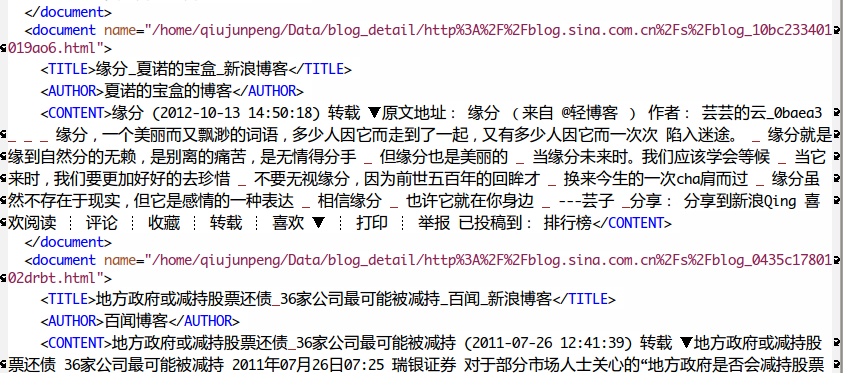
\includegraphics[width=0.8\textwidth]{xmloutput-1}
\end{figure}
\end{itemize}
\end{frame}

\begin{frame}[label=sec-3-6]{演示系统}
\begin{itemize}
\item 模板匹配演示系统的运行效果如下:
\begin{figure}[hb]
  \centering
  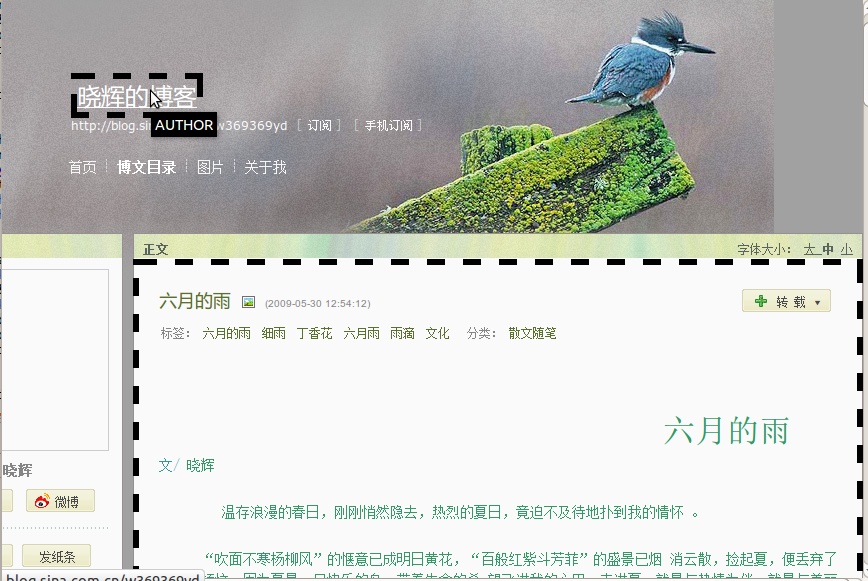
\includegraphics[width=0.8\textwidth]{demo-output-new}
\end{figure}
\end{itemize}
\end{frame}

%%% Local Variables: 
%%% mode: latex
%%% TeX-master: "../final_report_beamer"
%%% End: 
